\section{Erfaring}
En samlet liste af erfaringen de to kandidater har indenfor feltet hyttebombing indenfor Polyteknisk Forening:

\subsection{Studiestarten}
\begin{enumerate}
\item Vektor 2006 \cite{bib:url:Beret2007}
\item CSK 2007\cite{bib:url:Beret2007}
\item CSK 2008\cite{bib:url:Beret2008}
\item Vektor 2008\cite{bib:url:Beret2008}
\item CSK 2009\cite{bib:url:Beret2009}
\item Vektor 2009\cite{bib:url:Beret2009}
\end{enumerate}

\subsection{Madhold}
\begin{enumerate}
\item vOPtur 2008\cite{bib:url:Beret2008}
\item Rustur 2009\cite{bib:url:Beret2009}
\item hyttetur ELKO nystartende 2010\cite{bib:url:Beret2010}
\item S-husets hyttetur 2011\cite{bib:url:Beret2011}
\item OPtur 2011\cite{bib:url:Beret2011}
\item Rustur 2011\cite{bib:url:Beret2011}
\item hyttetur ELKO nystartende 2011\cite{bib:url:Beret2011}
\item S-husets hyttetur 2012
\end{enumerate}


\subsection{Arrangør af ture}

\begin{enumerate}
\item Rustur 2006\cite{bib:url:Beret2007}
\item HerreHyggeHyttetur ELKO 2007 \cite{bib:url:Beret2007}
\item OPtur 2007\cite{bib:url:Beret2007}
\item Rustur 2007\cite{bib:url:Beret2007}
\item HerreHyggeHyttetur ELKO 2008\cite{bib:url:Beret2008}
\item OPtur 2008\cite{bib:url:Beret2008}
\item Rustur 2008\cite{bib:url:Beret2008}
\item hyttetur ELKO nystartende 2008\cite{bib:url:Beret2008}
\item HerreHyggeHyttetur ELKO 2009\cite{bib:url:Beret2009}
\item OPtur 2009\cite{bib:url:Beret2009}
\item Rustur 2009\cite{bib:url:Beret2009}
\item hyttetur ELKO nystartende 2009\cite{bib:url:Beret2009}
\item HerreHyggeHyttetur ELKO 2011\cite{bib:url:Beret2011}
\item HerreHyggeHyttetur ELKO 2012
\end{enumerate}

\subsection{PF kompetancer}
\begin{enumerate}
\item Medlem ELKO 2006-2012\cite{bib:url:Beret2007},\cite{bib:url:Beret2008},\cite{bib:url:Beret2009},\cite{bib:url:Beret2010},\cite{bib:url:Beret2011}
\item Formand for ELKO rådet 2007-2009\cite{bib:url:Beret2007},\cite{bib:url:Beret2008},\cite{bib:url:Beret2009}
\item UddanelsesPolitisk Råd 2007-2012\cite{bib:url:Beret2007},\cite{bib:url:Beret2008},\cite{bib:url:Beret2009},\cite{bib:url:Beret2010},\cite{bib:url:Beret2011}
\item ISN Fotonik 2007-2012\cite{bib:url:Beret2007},\cite{bib:url:Beret2008},\cite{bib:url:Beret2009},\cite{bib:url:Beret2010},\cite{bib:url:Beret2011} , \cite{bib:url:ISNfoto}
\item Hegnet 2007->\cite{bib:url:Beret2007},\cite{bib:url:Beret2008},\cite{bib:url:Beret2009},\cite{bib:url:Beret2010},\cite{bib:url:Beret2011}
\item Hegnet Formand 2007-2008\cite{bib:url:Beret2007},\cite{bib:url:Beret2008}
\item Fællesrådet 2009+2011-2012\cite{bib:url:Beret2009},\cite{bib:url:Beret2010},\cite{bib:url:Beret2011}
\item Fællesrådets ForretningsUdvalg 2009-2012\cite{bib:url:Beret2009},\cite{bib:url:Beret2010},\cite{bib:url:Beret2011}
\item PF's Bestyrelse 2010\cite{bib:url:Beret2010}
\item Formand for ELKO rådet 2011-2012 \cite{bib:url:Beret2011}
\item Akademisk Råd (DTU) 2011-2012\cite{bib:url:Beret2011}
\end{enumerate}

\section{Kødpopularitet}


%\begin{tikzpicture}
%\begin{axis}[
%ybar,
%enlargelimits=0.15,
%legend style={at={(0.5,-0.15)},
%anchor=north,legend columns=-1},
%ylabel={\#participants},
%symbolic x coords={tool8,tool9,tool10},
%xtick=data,
%nodes near coords,
%nodes near coords align={vertical},
%]
%\addplot coordinates {(tool8,7) (tool9,9) (tool10,4)};
%\addplot coordinates {(tool8,4) (tool9,4) (tool10,4)};
%\addplot coordinates {(tool8,1) (tool9,1) (tool10,1)};
%\legend{used,understood,not understood}
%\end{axis}
%\end{tikzpicture}
Herunder er de mest gængse kødprodukter listet efter popularitet i følge En unavngiven kilde der følger miljøet tæt:\\
Bacon \cite{bib:url:WikiBacon} - ingen introduktion nødvendig\\
Kylling (Chicken) \cite{bib:url:WikiChicken} - Kød fra små fjerklædte dinosaurnedstammende dyr.\\
Kalkun (Turkey) \cite{bib:url:WikiTurkey}- Kød fra lidt større fjerklædte dinosaurnedstammende dyr. De flyver vist ikke så godt længere og er derfor nemme at fange med ene trefork\\ 
Svin (Pork) \cite{bib:url:WikiPork} - Kød der er en god bund i en fantastisk lagkage\\
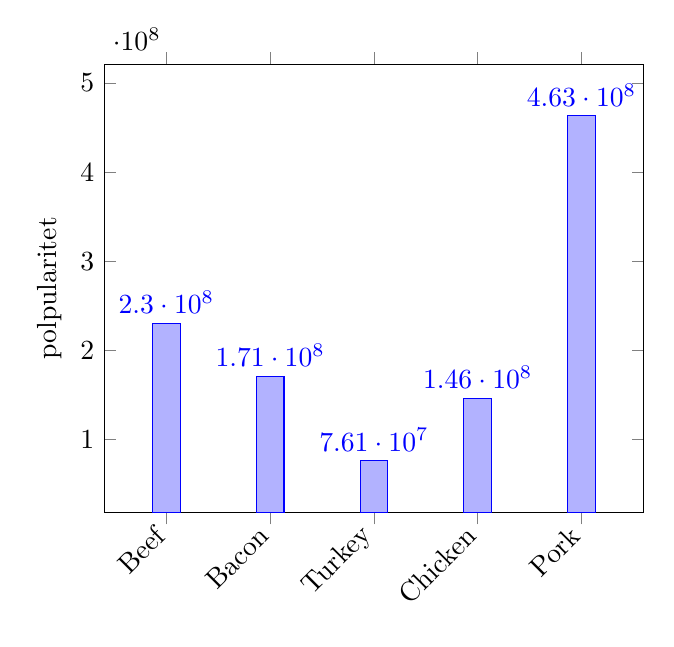
\begin{tikzpicture}
\begin{axis}[
ybar,
enlargelimits=0.15,
legend style={at={(0.5,-0.1)},
anchor=north,legend columns=-1},
ylabel={polpularitet},
symbolic x coords={Beef,	Bacon,	Turkey,	Chicken,	Pork},
xtick=data,
nodes near coords,
nodes near coords align={vertical},
x tick label style={rotate=45,anchor=east},
]
\addplot coordinates {(Beef,230000000) (Bacon,171000000) (Turkey,76100000) (Chicken,146000000) (Pork,463000000)};
\end{axis}
\end{tikzpicture}

En nærmere undersøgelse viser dog tydeligt Bacons posistion som svinets mest elskede kød:\\
Bacon \cite{bib:url:WikiBacon}\\
Flæskesteg \cite{bib:url:WikiRoastPork}\\
Ham \cite{bib:url:WikiHam}
Loin \cite{bib:url:WikiLoin}\\
Spam \cite{bib:url:WikiSpam}\\
Spare Ribs \cite{bib:url:WikiSpareRibs}\\
Mørbrad \cite{bib:url:WikiTenderLoin}
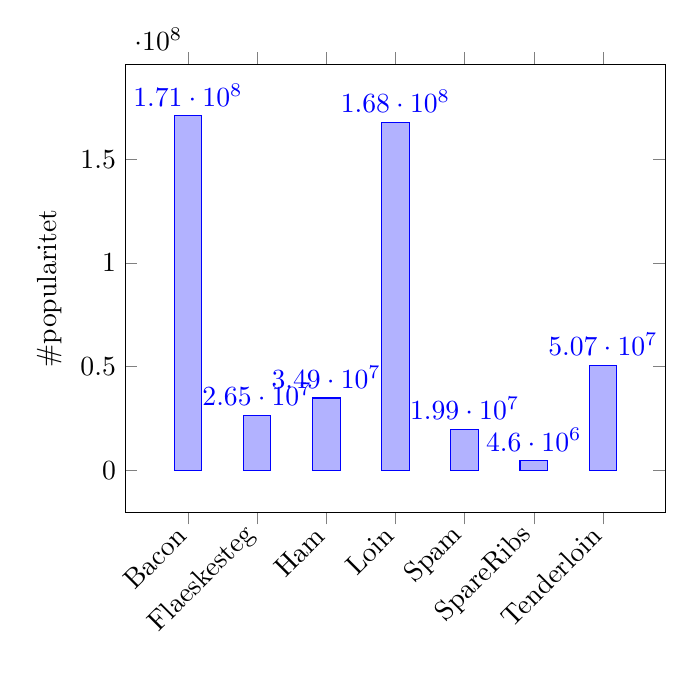
\begin{tikzpicture}
\begin{axis}[
ybar,
enlargelimits=0.15,
legend style={at={(0.5,-0.2)},
anchor=north,legend columns=-1},
ylabel={\#popularitet},
symbolic x coords={Bacon,Flaeskesteg,Ham,Loin,Spam,SpareRibs,Tenderloin},
xtick=data,
nodes near coords,
nodes near coords align={vertical},
x tick label style={rotate=45,anchor=east},
]
\addplot coordinates {(Bacon,171000000) (Flaeskesteg,26500000) (Ham,34900000) (Loin,168000000) (Spam,19900000)(SpareRibs,4600000)(Tenderloin,50700000)};
\end{axis}
\end{tikzpicture}

SPAM\footnote{Well, there's egg and bacon; egg sausage and bacon; egg and spam; egg bacon and spam; egg bacon sausage and spam; spam bacon sausage and spam; spam egg spam spam bacon and spam; spam sausage spam spam bacon spam tomato and spam; spam spam spam egg and spam; spam spam spam spam spam spam baked beans spam spam spam or Lobster Thermidor a Crevette with a mornay sauce served in a Provencale manner with shallots and aubergines garnished with truffle pate, brandy and with a fried egg on top and spam.}



\section{Hvad er Tha Bombs ikke}
\begin{enumerate}
\item Pædofil \cite{bib:url:Finn:Pedo}
\item Satan-tilbeder \cite{bib:url:Finn:Satan}
\item Dyrker sex med sovende kvinder \cite{bib:url:Finn:SovendeKvinder}
\item TV2 ansat \cite{bib:url:Finn:TV2}
\item Nazist\cite{bib:url:Finn:Nazist}
\end{enumerate}


Vi skal bruger DILD\cite{bib:url:Reklame:Dild}
\\
\\
Vi skal have en Anit Jehova Pæl \cite{bib:url:Reklame:Anti}
\\
\\
Tun i vand skal bruges \cite{bib:url:Reklame:Tun} rigeligt med tun i vand
\\
\\

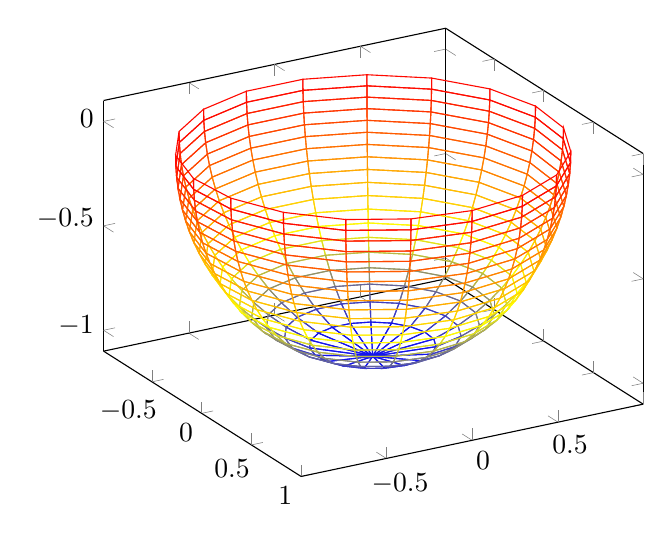
\begin{tikzpicture}
\begin{axis}[view={60}{30}]
\addplot3[mesh,z buffer=sort,
samples=20,domain=-1:0,y domain=0:2*pi]
({sqrt(1-x^2) * cos(deg(y))},
{sqrt( 1-x^2 ) * sin(deg(y))},
x);
\end{axis}
\end{tikzpicture}

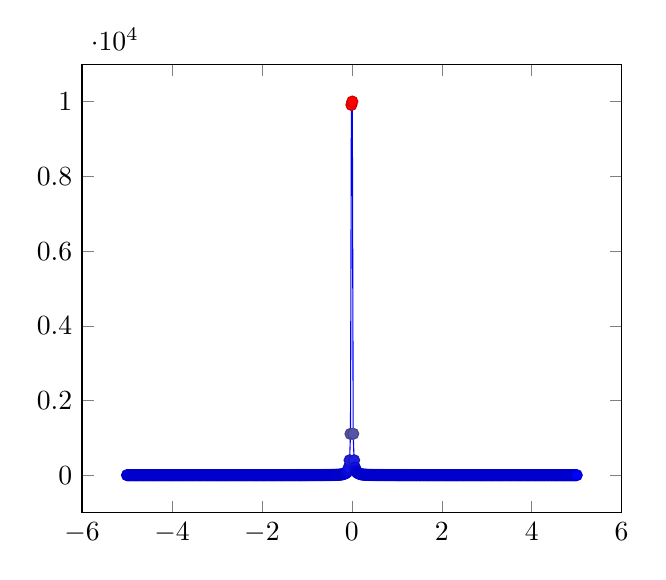
\begin{tikzpicture}
\begin{axis}
\addplot+[scatter,
samples=500,scatter src=y]
{x^-2};
\end{axis}
\end{tikzpicture}


